% !TEX TS-program = pdflatex
% !TEX encoding = UTF-8 Unicode

\documentclass[a4paper, titlepage=false, parskip=full-, 10pt]{scrartcl}

\usepackage[utf8]{inputenc}
\usepackage[T1]{fontenc}
\usepackage[english, ngerman]{babel}
\usepackage{babelbib}
\usepackage{hyperref}
\usepackage{listings}
\usepackage{framed}
\usepackage{color}
\usepackage{graphicx}
\usepackage[normalem]{ulem}
\usepackage{cancel}
\usepackage{array}
\usepackage{amsmath}
\usepackage{amssymb}
\usepackage{amsthm}
\usepackage{algorithm}
\usepackage{algorithmic}
\usepackage{geometry}
\usepackage{subfigure}
\geometry{a4paper, top=20mm, left=35mm, right=25mm, bottom=40mm}

\newcounter{tasknbr}
\setcounter{tasknbr}{1}
\newenvironment{task}[1]{{\bf Aufgabe \arabic {tasknbr}\stepcounter{tasknbr}} (#1):\begin{enumerate}}{\end{enumerate}}
\newcommand{\subtask}[1]{\item[#1)]}

% Listings -----------------------------------------------------------------------------
\definecolor{red}{rgb}{.8,.1,.2}
\definecolor{blue}{rgb}{.2,.3,.7}
\definecolor{lightyellow}{rgb}{1.,1.,.97}
\definecolor{gray}{rgb}{.7,.7,.7}
\definecolor{darkgreen}{rgb}{0,.5,.1}
\definecolor{darkyellow}{rgb}{1.,.7,.3}
\lstloadlanguages{C++,[Objective]C,Java}
\lstset{
escapeinside={§§}{§§},
basicstyle=\ttfamily\footnotesize\mdseries,
columns=fullflexible,
keywordstyle=\bfseries\color{blue},
commentstyle=\color{darkgreen},      
stringstyle=\color{red},
numbers=left,
numberstyle=\ttfamily\scriptsize\color{gray},
breaklines=true,
showstringspaces=false,
tabsize=4,
captionpos=b,
float=htb,
frame=tb,
frameshape={RYR}{y}{y}{RYR},
rulecolor=\color{black},
xleftmargin=15pt,
xrightmargin=4pt,
aboveskip=\bigskipamount,
belowskip=\bigskipamount,
backgroundcolor=\color{lightyellow},
extendedchars=true,
belowcaptionskip=15pt}

%% Enter current values here: %%
\newcommand{\lecture}{Robotik WS15/16}
\newcommand{\tutor}{}
\newcommand{\assignmentnbr}{9}
\newcommand{\students}{Julius Auer, Thomas Tegethoff}
%%-------------------------------------%%

\begin{document}  
{\small \textsl{\lecture \hfill \tutor}}
\hrule
\begin{center}
\textbf{Übungsblatt \assignmentnbr}\\
[\bigskipamount]
{\small \students}
\end{center}
\hrule

\begin{task}{A*-Suche}
\item[]
Da die Geschwindigkeit des Autos sowie die Schrittweite fest aber beliebig sind, haben wir einen kontinuierlichen Zustandsraum und lassen die CLOSED-Liste weg. Für den hier behandelten einfachen Fall wäre eine Implementierung für kontinuierliche Zustandsräume ein unverhältnismäßig großer Aufwand.

Die Auswahl der Nachbarn eines Knotens ist straight-forward: Knoten repräsentieren eine 3D-Pose des Autos, so dass es stets 3 Nachbarn gibt - je nachdem, ob man links / rechts / gar nicht einlenkt. Die neue Pose für den neuen Knoten ergibt sich daraus direkt.

Die tatsächlichen Kosten zwischen zwei Knoten entsprechen offensichtlich immer der Schrittweite.

Interessant ist die Wahl einer guten Heuristik. Es bieten sich hier natürlich Dubin-Kurven an. Als erste quick\&dirty Implementierung haben wir jedoch zunächst $L_2$-Distanzen als Heuristik verwendet und überraschend gute Ergebnisse erzielt: auch der ''lange'' Weg war in $<1s$ berechnet. Da es in der Aufgabe nicht näher spezifiert war haben wir deshlab - nichts für ungut - Dubin-Kurven nicht mehr implementiert. Zwischen den Jahren ist die Zeit immer eher knapp. Schade.

Um bei Verwendung einer $L_2$-Heuristik nicht mit dem Hindernis zu kollidieren, haben wir dieses artifiziell um die Schrittweite vergrößert. Dieses Vorgehen liefert natürlich keinen optimalen Pfad (im konkreten Fall dürfte jedoch kein Unterschied zu erkennen sein).

Ihr habt es uns durch den großzügen erlaubten Fehler recht einfach gemacht - ansonsten wären wir um Dubin ggf. nicht herum gekommen ...

Es seien im Folgenden: $e_p=2.5$ der zulässige Positionfehler, $e_o=1$ der zulässige Orientierungsfehler, $d$ die Schrittweite (als Vielfaches von $\pi$), $r=4$ der Radius des Wendekreises, $(x_o,y_o)\in\{\mathbb{R}^2|15\le x_o\le20\wedge -5\le y_o\le 20\}$ das Hindernis, $t=((x_t,y_t),(ox_t,oy_t))$ die Zielpose und $|O_d|$ die Größe der OPEN-Liste bei Schrittweite $d$.

\newpage
\subtask{a}
\begin{align*}
t&=((6,3),(0,1))\\
|O_1|&=3\\
|O_{0.5}|&=7
\end{align*}

\begin{figure}[!htpb]
\centering
\subfigure[$d=\pi$]{
  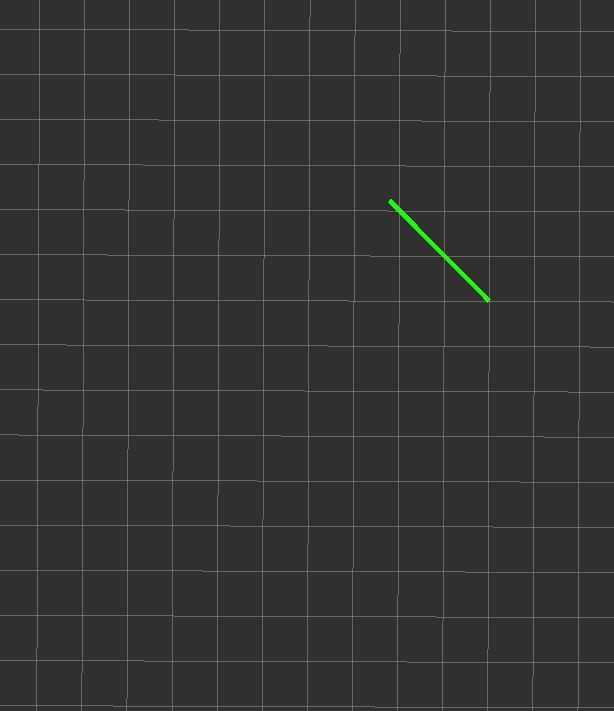
\includegraphics[width=0.3\linewidth]{capture_1-1}
}
\subfigure[$d=\frac{\pi}{2}$]{
  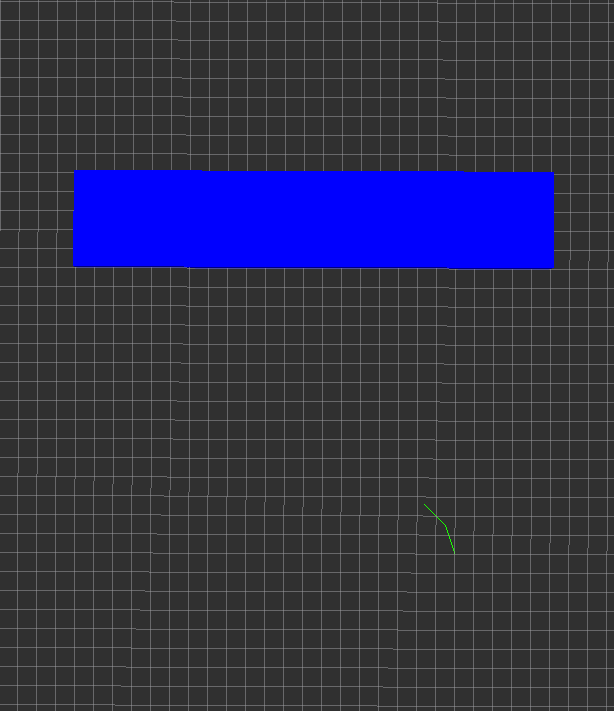
\includegraphics[width=0.3\linewidth]{capture_1-2}
}
\caption{Plot a}
\end{figure}

\subtask{b}
\begin{align*}
t&=((0,5),(0,-1))\\
|O_1|&=113\\
|O_{0.5}|&=3059
\end{align*}

\begin{figure}[!htpb]
\centering
\subfigure[$d=\pi$]{
  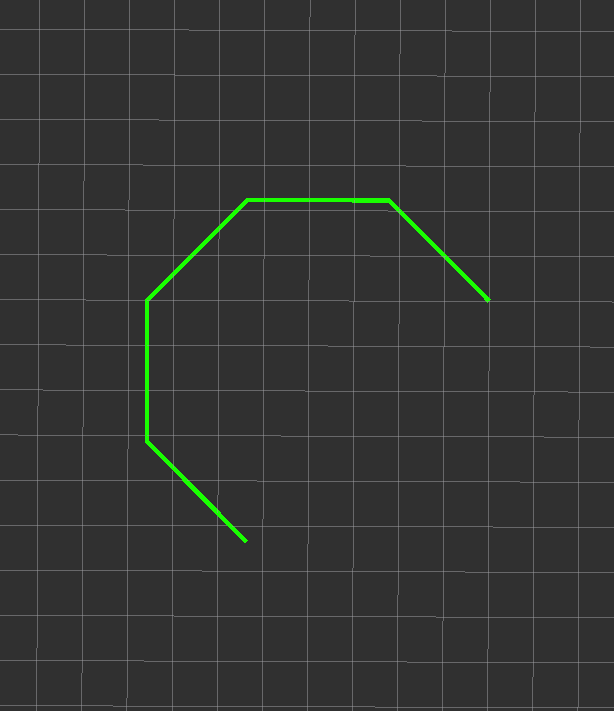
\includegraphics[width=0.3\linewidth]{capture_1-3}
}
\subfigure[$d=\frac{\pi}{2}$]{
  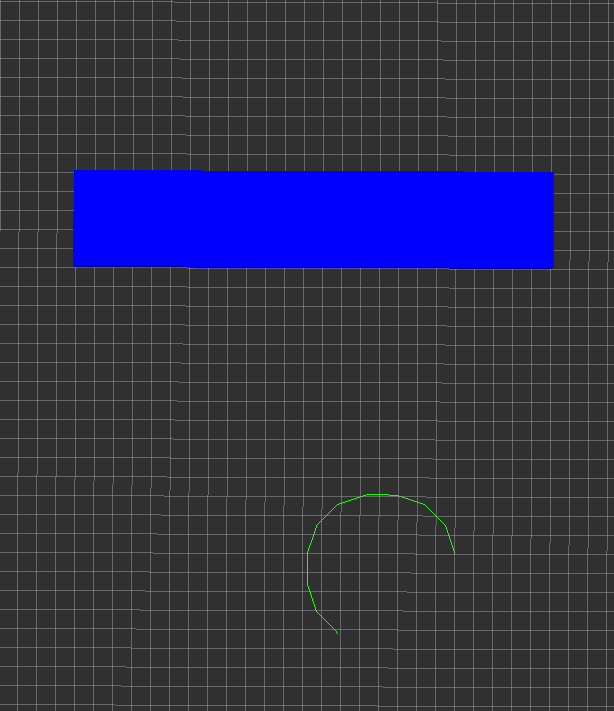
\includegraphics[width=0.3\linewidth]{capture_1-4}
}
\caption{Plot b}
\end{figure}

\newpage
\subtask{c}
\begin{align*}
t&=((0,5),(-1,0))\\
|O_1|&=13\\
|O_{0.5}|&=103
\end{align*}

\begin{figure}[!htpb]
\centering
\subfigure[$d=\pi$]{
  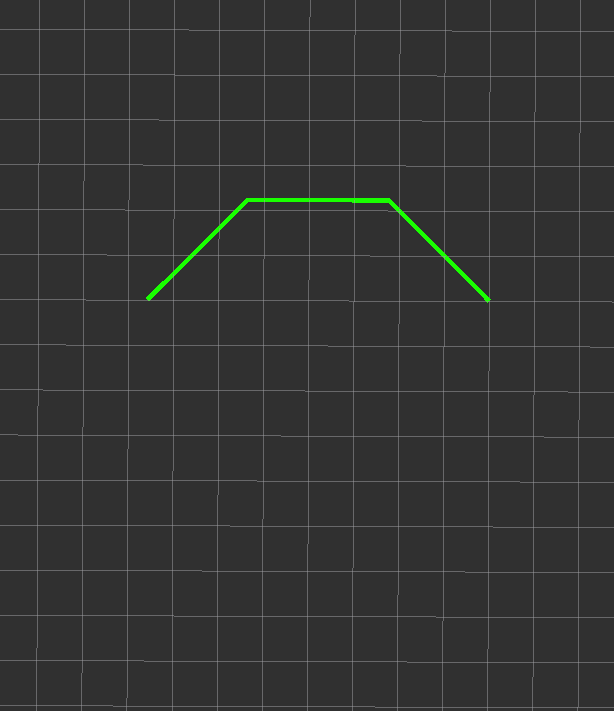
\includegraphics[width=0.3\linewidth]{capture_1-5}
}
\subfigure[$d=\frac{\pi}{2}$]{
  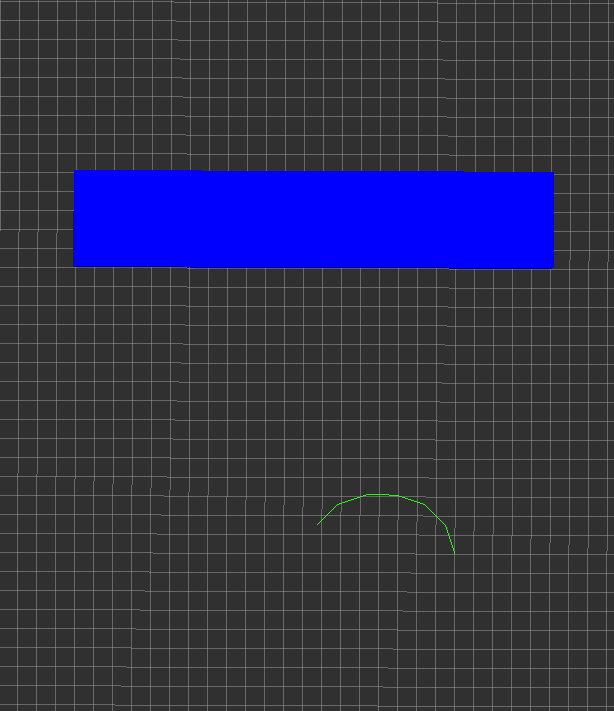
\includegraphics[width=0.3\linewidth]{capture_1-6}
}
\caption{Plot c}
\end{figure}

\subtask{d}
\begin{align*}
t&=((30,15),(1,0))\\
|O_1|&=1300\\
|O_{0.5}|&=3073656
\end{align*}
Die kleine Überschneidung mit dem Hindernis (rechts) ist lediglich auf die etwas dicker gezeichnete Linie zurückzuführen.

\begin{figure}[!htpb]
\centering
\subfigure[$d=\pi$]{
  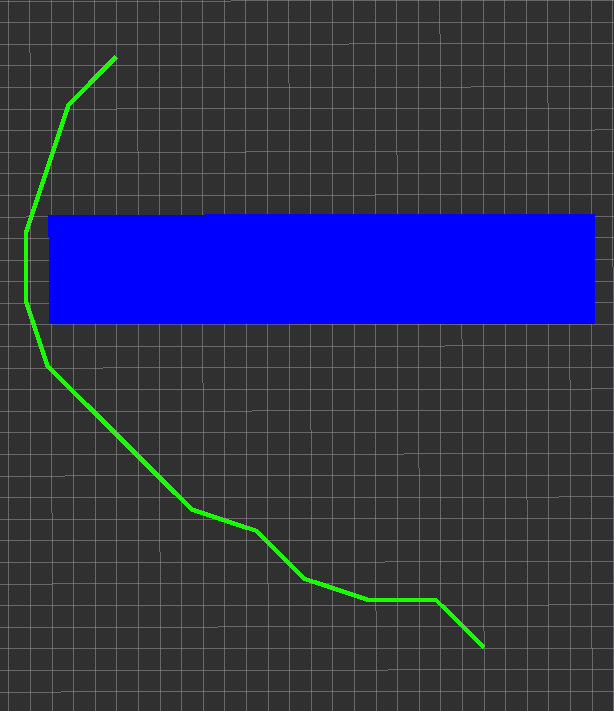
\includegraphics[width=0.3\linewidth]{capture_1-7}
}
\subfigure[$d=\frac{\pi}{2}$]{
  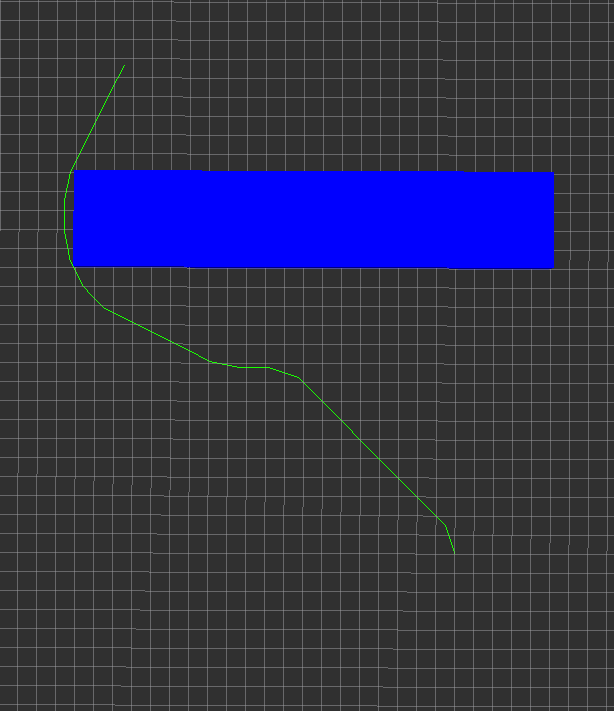
\includegraphics[width=0.3\linewidth]{capture_1-8}
}
\caption{Plot d}
\end{figure}
\end{task}
\end{document}